\section{Introducción}

\textbf{La productividad ocupa un lugar central en cualquier agenda de desarrollo.} La literatura económica sobre crecimiento ha mostrado que, en el largo plazo, la capacidad de sostener aumentos en los ingresos de los habitantes depende menos de acumular más capital o de incorporar más trabajadores y horas trabajadas, y más de producir mayor valor agregado con los recursos disponibles. En otras palabras, el crecimiento económico sostenido requiere aumentos de productividad.

\textbf{El objetivo de este informe es medir la evolución de la productividad laboral en Colombia entre 2010 y 2025.} Con este fin se combina el PIB por actividad económica reportado por el DANE y la información de ocupados y horas trabajadas de la Gran Encuesta Integrada de Hogares (GEIH). A partir de esa combinación se construyen dos indicadores complementarios: el \textbf{PIB por trabajador} y el \textbf{PIB por hora trabajada}. La distinción es importante porque el número de ocupados y las horas promedio no necesariamente crecen al mismo ritmo, lo cual hace que las conclusiones que se derivan de un indicador u otro no sean necesariamente las mismas.

\textbf{En Colombia, el PIB por hora trabajada ha crecido más que el PIB por trabajador}. Durante los últimos quince años la economía logró crecer a una tasa promedio de más del 3\% anual. Sin embargo, es importante desagregar los motivos de esa expansión. Mientras la población ocupada creció a más del 2\% anual, el PIB por trabajador aumentó apenas cerca de 1\% anual. Al mismo tiempo, las horas semanales promedio por trabajador disminuyeron casi 0,5\% anual. Esa reducción hace que el PIB por hora haya crecido más que el PIB por trabajador. En efecto, el crecimiento del PIB por hora fue de 1,5\% anual.

\textbf{Existe una gran dispersión en el crecimiento de la productividad de las grandes ramas de actividad económica.} Este informe no solo estudia la dinámica de la productividad agregada, sino también la productividad de las doce agrupaciones CIIU usadas por el DANE. Durante el periodo 2010--2025, actividades como información y comunicaciones alcanzaron un crecimiento anualizado del 4,5\% en el producto por hora trabajada, mientras que actividades como explotación de minas y canteras enfrentaron una reducción anualizada del 3,1\% en su producto por hora trabajada.

\textbf{Una pregunta central es si la ocupación creció en los sectores donde también creció la productividad.} Los resultados muestran que, entre 2010 y 2025, las actividades con el mayor aumento porcentual en el número de ocupados no fueron aquellas donde más creció el PIB por trabajador o el PIB por hora trabajada. Esto no necesariamente debe interpretarse como una señal de mala asignación de los ocupados, dado que algunas de las actividades con mayor crecimiento de la productividad partían de niveles relativamente bajos. Por esa razón, informes posteriores del Centro Javeriano de Competitividad estudiarán con más detalle la asignación de los factores de producción entre distintas actividades económicas, con el fin de estimar las potenciales ganancias de eficiencia que se alcanzarían al reducir las barreras que impiden que los recursos se asignen hacia sus usos más productivos.

\textbf{Después de esta introducción, el informe está organizado en cinco secciones adicionales.} La sección 2 presenta la metodología y la descomposición que permite separar el crecimiento del PIB entre ocupación, horas trabajadas y productividad por hora. La sección 3 describe la evolución agregada de la productividad laboral en Colombia. La sección 4 analiza las diferencias entre las doce agrupaciones sectoriales. La sección 5 estudia la relación entre crecimiento de la ocupación y crecimiento de la productividad a través de sectores. Finalmente, la sección 6 presenta las conclusiones.

\begin{comment}
\subsection{Comparación internacional: productividad laboral}

Antes de analizar la evolución del empleo y de los ingresos laborales en Colombia, conviene ubicar el desempeño del país en perspectiva internacional. Una forma sintética de hacerlo es comparar el PIB por trabajador, una medida amplia de productividad laboral que aproxima el valor agregado generado por cada persona ocupada. Aunque este indicador no captura todas las diferencias en calidad del empleo, informalidad, horas trabajadas o composición sectorial, permite establecer si el crecimiento colombiano ha sido suficiente para cerrar brechas frente a economías comparables y frente a referentes de mayor ingreso.

\begin{table}[H]
\centering
\caption{PIB por trabajador y crecimiento anualizado, 2010--2024}
\label{tab:pib_trabajador_internacional}
\begin{tabular}{lrrr}
\toprule
País & 2010 & 2024 & Crec. anualizado \\
\midrule
Costa Rica & 45.175 & 61.875 & 2,27\% \\
República Dominicana & 40.301 & 53.911 & 2,10\% \\
Perú & 22.321 & 29.844 & 2,10\% \\
Colombia & 32.469 & 40.363 & 1,57\% \\
Estados Unidos & 129.284 & 153.544 & 1,24\% \\
Chile & 55.677 & 63.924 & 0,99\% \\
Brasil & 39.603 & 41.441 & 0,32\% \\
México & 49.943 & 48.671 & -0,18\% \\
\bottomrule
\end{tabular}
\caption*{\footnotesize Nota: valores en dólares internacionales constantes de 2021 ajustados por paridad de poder adquisitivo (PPP). El crecimiento anualizado corresponde a la variación compuesta entre 2010 y 2024. Fuente: Banco Mundial, World Development Indicators, indicador \texttt{SL.GDP.PCAP.EM.KD}.}
\end{table}

\textbf{En perspectiva internacional, Colombia muestra un avance real de la productividad laboral, pero insuficiente para cerrar de manera clara sus brechas frente a varios pares regionales.} Entre 2010 y 2024, el PIB por trabajador en Colombia pasó de 32.469 a 40.363 dólares internacionales constantes de 2021, equivalente a un crecimiento anualizado de 1,57\%. Esta tasa supera la observada en Estados Unidos, Chile, Brasil y México durante el mismo período, un resultado que a primera vista puede parecer sorprendente. Sin embargo, debe interpretarse a la luz de los niveles iniciales: Estados Unidos y Chile partían de un PIB por trabajador sustancialmente más alto que Colombia, por lo que un crecimiento relativo menor es consistente con la idea, ampliamente documentada en la literatura económica, de que las economías con menor productividad inicial pueden crecer más rápido cuando tienen espacio para adoptar tecnologías, reorganizar procesos productivos y reasignar recursos hacia actividades de mayor valor agregado.

La comparación también muestra los límites de esa lectura optimista. Costa Rica y República Dominicana ya registraban en 2010 un PIB por trabajador superior al colombiano y, aun así, crecieron más rápido entre 2010 y 2024. Esto sugiere que el rezago de Colombia no se explica únicamente por su punto de partida, sino por la velocidad con la que transforma mejoras en empleo, capital humano, formalización y estructura productiva en aumentos sostenidos de productividad. En otras palabras, Colombia ha avanzado, pero no al ritmo necesario para converger con las economías latinoamericanas que han logrado combinar mayores niveles iniciales con una dinámica reciente más vigorosa.
\end{comment}


\section{Metodología y descomposición de la productividad}

\textbf{La medición de productividad laboral combina información de cuentas nacionales y de la GEIH.} El PIB anual se toma de las cuentas nacionales trimestrales del DANE por el enfoque de producción y se expresa en pesos constantes de 2015. Para cada año, el PIB anual corresponde a la suma de los cuatro trimestres. La población ocupada se calcula con los microdatos anuales de la GEIH, expandiendo a las personas ocupadas con su factor de expansión. Esta medida corresponde al número de ocupados representado por la encuesta en cada año; no es un dato de cierre de periodo, sino una medida anual comparable con los agregados laborales del DANE. En las validaciones previas del proyecto, esta serie fue contrastada con los totales oficiales de ocupación.

Las horas trabajadas también se construyen a partir de la GEIH. Para cada persona ocupada se toma el número de horas semanales trabajadas y se expande usando el mismo factor de expansión. La suma de esas horas semanales expandidas aproxima el total semanal de horas trabajadas en la economía; para obtener horas anuales, ese total se multiplica por 52 semanas. En el cálculo se excluyen reportes de horas no válidos y se conservan observaciones entre 1 y 112 horas semanales. Así, el PIB por hora trabajada divide el PIB anual por el total anual de horas trabajadas, mientras que el PIB por trabajador divide el PIB anual por el número de ocupados.

Para el análisis sectorial, el PIB del DANE y la información laboral de la GEIH deben estar expresados en las mismas actividades económicas. El PIB se reporta en doce agrupaciones CIIU Rev. 4 A.C. En la GEIH, los ocupados se asignan a esas mismas agrupaciones usando la variable de subrama de actividad económica disponible en la base procesada del proyecto. En algunos casos, varias subramas de la GEIH se agrupan para coincidir con las categorías del PIB; por ejemplo, comercio, transporte y alojamiento se presentan de manera conjunta, al igual que administración pública, educación y salud. Los resultados, los insumos y el código de replicación están disponibles en el repositorio del proyecto: \url{https://github.com/Kin-George/CJC-Monitor}.

\textbf{El crecimiento del PIB puede desagregarse entre ocupación, horas y productividad por hora.} En primer lugar, el PIB puede escribirse como el producto entre el PIB por trabajador y el número de ocupados:

\[
\text{PIB} = \text{Ocupados}\times
\left(\frac{\text{PIB}}{\text{Ocupados}}\right).
\]

A su vez, el PIB por trabajador combina dos elementos: cuánto se produce por cada hora trabajada y cuántas horas trabaja, en promedio, cada persona ocupada:

\[
\frac{\text{PIB}}{\text{Ocupados}} =
\left(\frac{\text{PIB}}{\text{Horas}}\right)
\times
\left(\frac{\text{Horas}}{\text{Ocupados}}\right).
\]

Combinando ambas expresiones, el PIB puede descomponerse en tres componentes:

\[
\text{PIB} = \text{Ocupados} \times \left(\frac{\text{PIB}}{\text{Horas}}\right) \times \left(\frac{\text{Horas}}{\text{Ocupados}}\right).
\]

%En términos de tasas de crecimiento anualizadas, esta identidad implica:

%\[
%1 + g_{\text{PIB}} =
%\left(1 + g_{\text{PIB/Horas}}\right)
%\left(1 + g_{\text{Horas/Trabajador}}\right)
%\left(1 + g_{\text{Ocupados}}\right).
%\]

%Para tasas moderadas, la misma relación puede leerse de manera aproximada como una suma:

%\[
%g_{\text{PIB}} \approx g_{\text{PIB/Horas}} + g_{\text{Horas/Trabajador}} + g_{\text{Ocupados}}.
%\]

Así, el crecimiento del producto puede provenir de tres márgenes: una mayor productividad por hora, más horas promedio por trabajador o un aumento en el número de ocupados. Esta descomposición permite distinguir si el crecimiento económico refleja principalmente una expansión del empleo o mejoras en la capacidad productiva del trabajo.

\section{Productividad laboral agregada}

\textbf{Esta sección presenta una primera mirada agregada a la productividad laboral en Colombia.} El objetivo es mostrar cómo evolucionaron, entre 2010 y 2025, el PIB real, el número de ocupados, las horas trabajadas y dos medidas complementarias de productividad: el PIB por trabajador y el PIB por hora trabajada. La lectura conjunta de estos indicadores permite distinguir si el crecimiento del producto proviene principalmente de más ocupados, de más horas por trabajador o de una mayor productividad por hora.

\begin{table}[H]
\centering
\caption{PIB, ocupados, horas y productividad laboral, 2010--2025}
\label{tab:ocupados_horas_resumen}
\small
\begin{tabular}{lrrr}
\toprule
Indicador & 2010 & 2025 & Crec. anualizado \\
\midrule
PIB real (Billones de pesos de 2015) & 640,2 & 1.021,1 & 3,16\% \\
Ocupados (Millones de personas) & 16,8 & 23,0 & 2,09\% \\
Horas semanales por trabajador (Horas por semana) & 46,8 & 43,7 & -0,45\% \\
PIB por trabajador (Millones de pesos de 2015 por ocupado) & 38,0 & 44,5 & 1,05\% \\
PIB por hora trabajada (Miles de pesos de 2015 por hora) & 15,6 & 19,6 & 1,51\% \\
\bottomrule
\end{tabular}
\caption*{\footnotesize Nota: PIB real en pesos constantes de 2015. Ocupados expandidos con el factor \texttt{fex}. Las horas semanales promedio se calculan como horas anuales totales divididas por ocupados y por 52 semanas. Se excluye 2020 por no contar con GEIH anual comparable en la base del proyecto. Fuente: cálculos propios con DANE, PIB trimestral por el enfoque de producción, y GEIH.}
\end{table}

El Cuadro \ref{tab:ocupados_horas_resumen} resume esta descomposición básica. Presenta, junto al PIB real, el número de ocupados, el PIB por trabajador, las horas semanales promedio por trabajador y el PIB por hora trabajada.

\textbf{La productividad laboral agregada aumentó entre 2010 y 2025, pero a un ritmo moderado.} El PIB por trabajador pasó de 38,0 a 44,5 millones de pesos constantes de 2015, equivalente a un crecimiento anualizado de 1,05\%. La medida por hora trabajada muestra una dinámica algo más favorable: aumentó de 15.625 a 19.563 pesos constantes de 2015 por hora, con una tasa anualizada de 1,51\%. La diferencia entre ambos indicadores es informativa: el número de ocupados creció con fuerza, de 16,8 a 23,0 millones de personas, pero las horas semanales promedio por trabajador descendieron de 46,8 a 43,7. Por esa razón, el denominador del PIB por hora crece menos que el denominador del PIB por trabajador, haciendo que la productividad por hora aumente más rápido que el PIB por trabajador.

Este resultado no debe interpretarse como una señal negativa por sí misma. Una reducción gradual de las horas trabajadas puede reflejar cambios en jornadas, composición ocupacional, regulación laboral o preferencias de oferta de trabajo. Sin embargo, sí es importante para la lectura de productividad: cuando se mide por trabajador, parte de la mejora queda amortiguada por el aumento del empleo; cuando se mide por hora, se observa con mayor claridad cuánto valor agregado produce la economía por unidad efectiva de tiempo trabajado.

La serie muestra una trayectoria ascendente hasta 2019, una discontinuidad en 2020 por ausencia de GEIH anual comparable en la base del proyecto, y un salto marcado en 2021. Este comportamiento debe interpretarse con cautela: después de la pandemia, el PIB se recuperó más rápido que el empleo y las horas trabajadas, elevando mecánicamente las medidas de productividad. En los años posteriores, el indicador se moderó, pero se mantuvo por encima de los niveles de 2010. Así, el mensaje central no es de estancamiento absoluto, sino de avance insuficiente: Colombia produce más por trabajador y por hora que al inicio de la década, pero la velocidad de mejora sigue siendo limitada frente al tamaño de las brechas productivas documentadas en la comparación internacional.

\section{Productividad laboral por sectores CIIU}

La productividad agregada oculta diferencias sustanciales entre ramas de actividad. Para examinarlas, se cruza el PIB sectorial del DANE, reportado en 12 agrupaciones CIIU Rev. 4 A.C., con los ocupados y horas de la GEIH armonizados a esas mismas agrupaciones mediante la variable de subrama homologada del proyecto. Esta aproximación permite estimar, para cada sector, el PIB por trabajador y el PIB por hora trabajada entre 2010 y 2025.

\begin{table}[H]
\centering
\caption{Productividad laboral por sector CIIU, 2010--2025}
\label{tab:pib_geih_productividad_sector}
\scriptsize
\begin{tabular}{lrrrrrr}
\toprule
& \multicolumn{3}{c}{PIB por trabajador} & \multicolumn{3}{c}{PIB por hora} \\
\cmidrule(lr){2-4}\cmidrule(lr){5-7}
Sector & 2010 & 2025 & Crec. & 2010 & 2025 & Crec. \\
\midrule
Artes, otros servicios y hogares & 10,4 & 24,2 & 5,79\% & 4.726 & 11.643 & 6,20\% \\
Información y comunicaciones & 45,3 & 78,6 & 3,74\% & 17.586 & 34.042 & 4,50\% \\
Agropecuario & 13,5 & 20,4 & 2,79\% & 5.778 & 9.361 & 3,27\% \\
Adm. pública, educación y salud & 43,6 & 58,4 & 1,96\% & 19.391 & 26.080 & 2,00\% \\
Financieras & 101,0 & 124,5 & 1,40\% & 42.977 & 54.186 & 1,56\% \\
Comercio, transporte y alojamiento & 19,9 & 24,1 & 1,28\% & 7.626 & 10.118 & 1,90\% \\
Manufactura & 41,1 & 45,0 & 0,61\% & 16.944 & 19.530 & 0,95\% \\
Inmobiliarias & 280,0 & 284,6 & 0,11\% & 105.347 & 119.543 & 0,85\% \\
Profesionales y administrativas & 56,6 & 42,4 & -1,90\% & 25.961 & 20.619 & -1,52\% \\
Construcción & 41,8 & 26,1 & -3,08\% & 16.429 & 11.011 & -2,63\% \\
Minas & 200,8 & 115,8 & -3,60\% & 77.628 & 48.441 & -3,09\% \\
Servicios públicos & 180,1 & 99,5 & -3,88\% & 71.289 & 43.452 & -3,25\% \\
\bottomrule
\end{tabular}
\caption*{\footnotesize Nota: PIB por trabajador en millones de pesos constantes de 2015 por ocupado; PIB por hora en pesos constantes de 2015 por hora trabajada. Sectores según 12 agrupaciones CIIU Rev. 4 A.C. del DANE; ocupados y horas se agregan desde GEIH usando la homologación de subramas del proyecto. Se excluyen organizaciones extraterritoriales del cruce sectorial por no hacer parte de las 12 agrupaciones. Fuente: cálculos propios con DANE y GEIH.}
\end{table}

\textbf{La descomposición sectorial revela que el desempeño agregado combina sectores con ganancias rápidas de productividad y sectores con deterioros importantes.} Las mayores tasas de crecimiento del PIB por trabajador se observan en artes, otros servicios y hogares (5,79\% anual), información y comunicaciones (3,74\%) y agropecuario (2,79\%). En estos casos, la productividad por hora crece incluso más rápido que la productividad por trabajador, lo que sugiere que la mejora no solo refleja cambios en el número de ocupados, sino también una mayor producción por unidad efectiva de tiempo trabajado. El caso de información y comunicaciones es especialmente relevante para la agenda de competitividad: parte de un nivel medio-alto en 2010 y aun así registra una expansión acelerada, consistente con el peso creciente de actividades digitales, telecomunicaciones, software y servicios intensivos en conocimiento.

En contraste, servicios públicos, minas, construcción y actividades profesionales y administrativas muestran caídas del PIB por trabajador y del PIB por hora. Estos resultados deben leerse con prudencia, pues mezclan cambios en valor agregado real, empleo, horas y composición interna de cada agrupación. Sin embargo, sí apuntan a una conclusión sustantiva: no todos los sectores que absorben empleo están elevando su productividad al mismo ritmo, y algunos sectores de alta productividad inicial han perdido terreno relativo. Minas y servicios públicos siguen registrando niveles altos de PIB por trabajador frente al promedio nacional, pero su crecimiento negativo indica que la ventaja inicial se redujo durante el período.

La heterogeneidad sectorial refuerza una idea central del informe: el problema de productividad en Colombia no es solo agregado, sino de estructura productiva. La economía combina sectores modernos con capacidad de expansión, sectores intensivos en empleo de baja productividad y ramas con altos niveles iniciales pero bajo dinamismo reciente. Por ello, una agenda de productividad laboral no puede limitarse a aumentar la ocupación o mejorar los ingresos laborales promedio; debe también facilitar la reasignación de trabajadores hacia actividades de mayor valor agregado, elevar la productividad dentro de los sectores de mayor absorción laboral y cerrar las brechas de capital humano, tecnología y formalización que impiden que el crecimiento sectorial se traduzca en mejores ingresos.

%La lectura por doce agrupaciones es la columna vertebral del análisis sectorial. Dentro de cada subsección se incluye, cuando corresponde, un zoom a 25 agrupaciones para mostrar qué ocurre al abrir la actividad amplia en subsectores más específicos. En las actividades donde la apertura a 25 agrupaciones coincide con la de 12, pero la apertura a 61 sí ofrece mayor detalle, el zoom usa esa desagregación más fina.
\textbf{A continuación se presenta la descomposición del crecimiento de cada una de las doce agrupaciones de actividad económica CIIU.} En particular, se presenta el PIB real de la actividad, el número de ocupados, el PIB por trabajador, las horas semanales promedio por trabajador y el PIB por hora trabajada para los años 2010 y 2025. La lectura conjunta de estas variables permite distinguir si los cambios de productividad responden principalmente al dinamismo del producto, a variaciones en el empleo, a cambios en las horas trabajadas o a una combinación de estos factores. Las descripciones siguen la agregación usada por el DANE; por eso, en algunos casos reúnen actividades económicas muy distintas dentro de una misma agrupación.

\subsection{Agropecuario}

Esta agrupación reúne agricultura, ganadería, caza, silvicultura y pesca.

\begin{table}[H]
\centering
\caption{Agropecuario: PIB, ocupados, horas y productividad laboral, 2010--2025}
\label{tab:sector_a_productividad}
\small
\begin{tabular}{lrrr}
\toprule
Indicador & 2010 & 2025 & Crec. anual \\
\midrule
PIB real  (Billones de pesos de 2015) & 39,9 & 63,9 & 3,18\% \\
Ocupados (Millones) & 3,0 & 3,1 & 0,38\% \\
PIB por trabajador (Millones de pesos de 2015) & 13,5 & 20,4 & 2,79\% \\
Horas semanales por trabajador & 45,0 & 42,0 & -0,46\% \\
PIB por hora trabajada (Miles de pesos de 2015) & 5,8 & 9,4 & 3,27\% \\
\bottomrule
\end{tabular}
\end{table}

\textbf{Frente al agregado nacional, la comparación variable por variable muestra diferencias relevantes.} El PIB real de la actividad registró una tasa anualizada de 3,18\%, muy cerca del agregado (3,16\%). La ocupación en la actividad registró una tasa anualizada de 0,38\%, por debajo del agregado (2,09\%). El PIB por trabajador registró una tasa anualizada de 2,79\%, por encima del agregado (1,05\%). Las horas semanales por trabajador registraron una tasa anualizada de -0,46\%, muy cerca de la caída agregada (-0,45\%). El PIB por hora trabajada registró una tasa anualizada de 3,27\%, por encima del agregado (1,51\%).

\textbf{En niveles de 2025, el tamaño relativo y la productividad de la actividad económica también importan.} La actividad representó 6,3\% del PIB real agregado, con 63,9 billones de pesos de 2015, y concentró 13,6\% de los ocupados, con 3,1 millones de personas. El PIB por trabajador fue 20,4 millones de pesos de 2015 por ocupado, por debajo del agregado (44,5 millones). Las horas semanales por trabajador fueron 42,0, muy cerca del agregado (43,7). El PIB por hora trabajada fue 9,4 mil pesos de 2015 por hora, por debajo del agregado (19,6 mil).

\textbf{Zoom a 61 agrupaciones.} En agropecuario, la apertura a 25 agrupaciones coincide con la agrupación de 12. Por eso, el zoom usa la apertura a 61 agrupaciones, que permite mirar subactividades más específicas.

\begin{table}[H]
\centering
\caption{Agropecuario: apertura de productividad laboral a 61 agrupaciones, 2010--2025}
\label{tab:sector_a_zoom61}
\scriptsize
\begin{tabular}{p{0.40\textwidth}rrrr}
\toprule
Actividad económica & PIB/trab. 2025 & Crec. & PIB/hora 2025 & Crec. \\
\midrule
Silvicultura & 70,2 & 5,15\% & 32,9 & 6,27\% \\
Pesca y acuicultura & 24,6 & 4,79\% & 10,9 & 5,75\% \\
Cultivos y apoyo agropecuario; Café; Ganadería & 19,9 & 2,74\% & 9,1 & 3,19\% \\
\bottomrule
\end{tabular}
\caption*{\footnotesize Nota: PIB por trabajador en millones de pesos constantes de 2015; PIB por hora en miles de pesos constantes de 2015. Cuando la GEIH no separa ocupados y horas al mismo nivel de las cuentas nacionales, se agrupan las subactividades del DANE hasta el nivel laboral comparable. Fuente: cálculos propios con DANE y GEIH.}
\end{table}

En esta apertura, el mayor crecimiento del PIB por trabajador se observa en Silvicultura (5,15\%), mientras que el menor se registra en Cultivos y apoyo agropecuario; Café; Ganadería (2,74\%). Por hora trabajada, el mejor desempeño corresponde a Silvicultura (6,27\%) y el más rezagado a Cultivos y apoyo agropecuario; Café; Ganadería (3,19\%).

\subsection{Minas}

Esta agrupación reúne explotación de minas y canteras. En la CIIU Rev. 4 A.C. corresponde a B; divisiones 05--09.

\begin{table}[H]
\centering
\caption{Minas: PIB, ocupados, horas y productividad laboral, 2010--2025}
\label{tab:sector_b_productividad}
\small
\begin{tabular}{lrrr}
\toprule
Indicador & 2010 & 2025 & Crec. anual \\
\midrule
PIB real  (Billones de pesos de 2015) & 38,4 & 34,7 & -0,67\% \\
Ocupados (Millones) & 0,2 & 0,3 & 3,04\% \\
PIB por trabajador (Millones de pesos de 2015) & 200,8 & 115,8 & -3,60\% \\
Horas semanales por trabajador & 49,7 & 46,0 & -0,52\% \\
PIB por hora trabajada (Miles de pesos de 2015) & 77,6 & 48,4 & -3,09\% \\
\bottomrule
\end{tabular}
\end{table}

\textbf{Frente al agregado nacional, la comparación variable por variable muestra diferencias relevantes.} El PIB real de la actividad registró una tasa anualizada de -0,67\%, por debajo del agregado (3,16\%). La ocupación en la actividad registró una tasa anualizada de 3,04\%, por encima del agregado (2,09\%). El PIB por trabajador registró una tasa anualizada de -3,60\%, por debajo del agregado (1,05\%). Las horas semanales por trabajador registraron una tasa anualizada de -0,52\%, muy cerca de la caída agregada (-0,45\%). El PIB por hora trabajada registró una tasa anualizada de -3,09\%, por debajo del agregado (1,51\%).

\textbf{En niveles de 2025, el tamaño relativo y la productividad de la actividad económica también importan.} La actividad representó 3,4\% del PIB real agregado, con 34,7 billones de pesos de 2015, y concentró 1,3\% de los ocupados, con 0,3 millones de personas. El PIB por trabajador fue 115,8 millones de pesos de 2015 por ocupado, por encima del agregado (44,5 millones). Las horas semanales por trabajador fueron 46,0, por encima del agregado (43,7). El PIB por hora trabajada fue 48,4 mil pesos de 2015 por hora, por encima del agregado (19,6 mil).

\textbf{Zoom a 61 agrupaciones.} En minas, la apertura a 25 agrupaciones coincide con la agrupación de 12. Por eso, el zoom usa la apertura a 61 agrupaciones, que permite mirar subactividades más específicas.

\begin{table}[H]
\centering
\caption{Minas: apertura de productividad laboral a 61 agrupaciones, 2010--2025}
\label{tab:sector_b_zoom61}
\scriptsize
\begin{tabular}{p{0.40\textwidth}rrrr}
\toprule
Actividad económica & PIB/trab. 2025 & Crec. & PIB/hora 2025 & Crec. \\
\midrule
Carbón; Petróleo, gas y apoyo conexo; Apoyo a otras actividades mineras & 308,0 & -2,44\% & 124,1 & -1,90\% \\
Minerales metalíferos; Otras minas y canteras & 22,1 & -5,13\% & 9,4 & -4,68\% \\
\bottomrule
\end{tabular}
\caption*{\footnotesize Nota: PIB por trabajador en millones de pesos constantes de 2015; PIB por hora en miles de pesos constantes de 2015. Cuando la GEIH no separa ocupados y horas al mismo nivel de las cuentas nacionales, se agrupan las subactividades del DANE hasta el nivel laboral comparable. Fuente: cálculos propios con DANE y GEIH.}
\end{table}

En esta apertura, el mayor crecimiento del PIB por trabajador se observa en Carbón; Petróleo, gas y apoyo conexo; Apoyo a otras actividades mineras (-2,44\%), mientras que el menor se registra en Minerales metalíferos; Otras minas y canteras (-5,13\%). Por hora trabajada, el mejor desempeño corresponde a Carbón; Petróleo, gas y apoyo conexo; Apoyo a otras actividades mineras (-1,90\%) y el más rezagado a Minerales metalíferos; Otras minas y canteras (-4,68\%).

\subsection{Manufactura}

Esta agrupación reúne industrias manufactureras. En la CIIU Rev. 4 A.C. corresponde a C; divisiones 10--33.

\begin{table}[H]
\centering
\caption{Manufactura: PIB, ocupados, horas y productividad laboral, 2010--2025}
\label{tab:sector_c_productividad}
\small
\begin{tabular}{lrrr}
\toprule
Indicador & 2010 & 2025 & Crec. anual \\
\midrule
PIB real  (Billones de pesos de 2015) & 88,0 & 113,1 & 1,69\% \\
Ocupados (Millones) & 2,1 & 2,5 & 1,07\% \\
PIB por trabajador (Millones de pesos de 2015) & 41,1 & 45,0 & 0,61\% \\
Horas semanales por trabajador & 46,6 & 44,3 & -0,34\% \\
PIB por hora trabajada (Miles de pesos de 2015) & 16,9 & 19,5 & 0,95\% \\
\bottomrule
\end{tabular}
\end{table}

\textbf{Frente al agregado nacional, la comparación variable por variable muestra diferencias relevantes.} El PIB real de la actividad registró una tasa anualizada de 1,69\%, por debajo del agregado (3,16\%). La ocupación en la actividad registró una tasa anualizada de 1,07\%, por debajo del agregado (2,09\%). El PIB por trabajador registró una tasa anualizada de 0,61\%, por debajo del agregado (1,05\%). Las horas semanales por trabajador registraron una tasa anualizada de -0,34\%, muy cerca de la caída agregada (-0,45\%). El PIB por hora trabajada registró una tasa anualizada de 0,95\%, por debajo del agregado (1,51\%).

\textbf{En niveles de 2025, el tamaño relativo y la productividad de la actividad económica también importan.} La actividad representó 11,1\% del PIB real agregado, con 113,1 billones de pesos de 2015, y concentró 10,9\% de los ocupados, con 2,5 millones de personas. El PIB por trabajador fue 45,0 millones de pesos de 2015 por ocupado, muy cerca del agregado (44,5 millones). Las horas semanales por trabajador fueron 44,3, muy cerca del agregado (43,7). El PIB por hora trabajada fue 19,5 mil pesos de 2015 por hora, muy cerca del agregado (19,6 mil).

\textbf{Zoom a 25 agrupaciones.} Dentro de manufactura, la apertura a 25 agrupaciones permite ver diferencias que el promedio de la actividad oculta.

\begin{table}[H]
\centering
\caption{Manufactura: apertura de productividad laboral a 25 agrupaciones, 2010--2025}
\label{tab:sector_c_zoom25}
\scriptsize
\begin{tabular}{p{0.40\textwidth}rrrr}
\toprule
Actividad económica & PIB/trab. 2025 & Crec. & PIB/hora 2025 & Crec. \\
\midrule
Alimentos, bebidas y tabaco & 50,8 & 1,60\% & 21,8 & 1,70\% \\
Madera, papel e impresión & 46,9 & 1,46\% & 21,8 & 2,21\% \\
Textiles, confecciones y cuero & 17,5 & 0,74\% & 7,8 & 1,19\% \\
Metalurgia, maquinaria y equipo & 48,8 & 0,53\% & 20,5 & 1,00\% \\
Refinación, químicos y minerales & 106,6 & -0,75\% & 44,8 & -0,30\% \\
Muebles y otras manufactureras & 17,4 & -1,31\% & 7,6 & -1,06\% \\
\bottomrule
\end{tabular}
\caption*{\footnotesize Nota: PIB por trabajador en millones de pesos constantes de 2015; PIB por hora en miles de pesos constantes de 2015. Fuente: cálculos propios con DANE y GEIH.}
\end{table}

En esta apertura, el mayor crecimiento del PIB por trabajador se observa en Alimentos, bebidas y tabaco (1,60\%), mientras que el menor se registra en Muebles y otras manufactureras (-1,31\%). Por hora trabajada, el mejor desempeño corresponde a Madera, papel e impresión (2,21\%) y el más rezagado a Muebles y otras manufactureras (-1,06\%).

\subsection{Servicios públicos}

Esta agrupación reúne suministro de electricidad, gas, vapor y aire acondicionado; distribución de agua; evacuación y tratamiento de aguas residuales, gestión de desechos y actividades de saneamiento ambiental. En la CIIU Rev. 4 A.C. corresponde a D y E; divisiones 35--39.

\begin{table}[H]
\centering
\caption{Servicios públicos: PIB, ocupados, horas y productividad laboral, 2010--2025}
\label{tab:sector_d_e_productividad}
\small
\begin{tabular}{lrrr}
\toprule
Indicador & 2010 & 2025 & Crec. anual \\
\midrule
PIB real  (Billones de pesos de 2015) & 21,9 & 30,3 & 2,18\% \\
Ocupados (Millones) & 0,1 & 0,3 & 6,30\% \\
PIB por trabajador (Millones de pesos de 2015) & 180,1 & 99,5 & -3,88\% \\
Horas semanales por trabajador & 48,6 & 44,0 & -0,65\% \\
PIB por hora trabajada (Miles de pesos de 2015) & 71,3 & 43,5 & -3,25\% \\
\bottomrule
\end{tabular}
\end{table}

\textbf{Frente al agregado nacional, la comparación variable por variable muestra diferencias relevantes.} El PIB real de la actividad registró una tasa anualizada de 2,18\%, por debajo del agregado (3,16\%). La ocupación en la actividad registró una tasa anualizada de 6,30\%, por encima del agregado (2,09\%). El PIB por trabajador registró una tasa anualizada de -3,88\%, por debajo del agregado (1,05\%). Las horas semanales por trabajador registraron una tasa anualizada de -0,65\%, una caída más pronunciada que la del agregado (-0,45\%). El PIB por hora trabajada registró una tasa anualizada de -3,25\%, por debajo del agregado (1,51\%).

\textbf{En niveles de 2025, el tamaño relativo y la productividad de la actividad económica también importan.} La actividad representó 3,0\% del PIB real agregado, con 30,3 billones de pesos de 2015, y concentró 1,3\% de los ocupados, con 0,3 millones de personas. El PIB por trabajador fue 99,5 millones de pesos de 2015 por ocupado, por encima del agregado (44,5 millones). Las horas semanales por trabajador fueron 44,0, muy cerca del agregado (43,7). El PIB por hora trabajada fue 43,5 mil pesos de 2015 por hora, por encima del agregado (19,6 mil).

\textbf{Zoom a 25 agrupaciones.} Dentro de servicios públicos, la apertura a 25 agrupaciones permite ver diferencias que el promedio de la actividad oculta.

\begin{table}[H]
\centering
\caption{Servicios públicos: apertura de productividad laboral a 25 agrupaciones, 2010--2025}
\label{tab:sector_d_e_zoom25}
\scriptsize
\begin{tabular}{p{0.40\textwidth}rrrr}
\toprule
Actividad económica & PIB/trab. 2025 & Crec. & PIB/hora 2025 & Crec. \\
\midrule
Electricidad, gas y vapor & 262,2 & -0,13\% & 109,6 & 0,28\% \\
Agua, saneamiento y desechos & 37,9 & -6,64\% & 16,9 & -5,96\% \\
\bottomrule
\end{tabular}
\caption*{\footnotesize Nota: PIB por trabajador en millones de pesos constantes de 2015; PIB por hora en miles de pesos constantes de 2015. Fuente: cálculos propios con DANE y GEIH.}
\end{table}

En esta apertura, el mayor crecimiento del PIB por trabajador se observa en Electricidad, gas y vapor (-0,13\%), mientras que el menor se registra en Agua, saneamiento y desechos (-6,64\%). Por hora trabajada, el mejor desempeño corresponde a Electricidad, gas y vapor (0,28\%) y el más rezagado a Agua, saneamiento y desechos (-5,96\%).

\subsection{Construcción}

Esta agrupación reúne construcción. En la CIIU Rev. 4 A.C. corresponde a F; divisiones 41--43.

\begin{table}[H]
\centering
\caption{Construcción: PIB, ocupados, horas y productividad laboral, 2010--2025}
\label{tab:sector_f_productividad}
\small
\begin{tabular}{lrrr}
\toprule
Indicador & 2010 & 2025 & Crec. anual \\
\midrule
PIB real  (Billones de pesos de 2015) & 40,0 & 41,3 & 0,21\% \\
Ocupados (Millones) & 1,0 & 1,6 & 3,39\% \\
PIB por trabajador (Millones de pesos de 2015) & 41,8 & 26,1 & -3,08\% \\
Horas semanales por trabajador & 48,9 & 45,7 & -0,46\% \\
PIB por hora trabajada (Miles de pesos de 2015) & 16,4 & 11,0 & -2,63\% \\
\bottomrule
\end{tabular}
\end{table}

\textbf{Frente al agregado nacional, la comparación variable por variable muestra diferencias relevantes.} El PIB real de la actividad registró una tasa anualizada de 0,21\%, por debajo del agregado (3,16\%). La ocupación en la actividad registró una tasa anualizada de 3,39\%, por encima del agregado (2,09\%). El PIB por trabajador registró una tasa anualizada de -3,08\%, por debajo del agregado (1,05\%). Las horas semanales por trabajador registraron una tasa anualizada de -0,46\%, muy cerca de la caída agregada (-0,45\%). El PIB por hora trabajada registró una tasa anualizada de -2,63\%, por debajo del agregado (1,51\%).

\textbf{En niveles de 2025, el tamaño relativo y la productividad de la actividad económica también importan.} La actividad representó 4,0\% del PIB real agregado, con 41,3 billones de pesos de 2015, y concentró 6,9\% de los ocupados, con 1,6 millones de personas. El PIB por trabajador fue 26,1 millones de pesos de 2015 por ocupado, por debajo del agregado (44,5 millones). Las horas semanales por trabajador fueron 45,7, muy cerca del agregado (43,7). El PIB por hora trabajada fue 11,0 mil pesos de 2015 por hora, por debajo del agregado (19,6 mil).

\textbf{Zoom a 25 agrupaciones.} El DANE abre construcción en edificaciones, obras civiles y actividades especializadas de construcción. Sin embargo, la GEIH histórica comparable no permite separar ocupados y horas entre esas tres subactividades. Por esa razón, no se presenta un cuadro de PIB por trabajador o PIB por hora a este nivel. La medición comparable corresponde al total de construcción.

\subsection{Comercio, transporte y alojamiento}

Esta agrupación reúne comercio al por mayor y al por menor; reparación de vehículos automotores y motocicletas; transporte y almacenamiento; alojamiento y servicios de comida. En la CIIU Rev. 4 A.C. corresponde a G, H e I; divisiones 45--56.

\begin{table}[H]
\centering
\caption{Comercio, transporte y alojamiento: PIB, ocupados, horas y productividad laboral, 2010--2025}
\label{tab:sector_g_h_i_productividad}
\small
\begin{tabular}{lrrr}
\toprule
Indicador & 2010 & 2025 & Crec. anual \\
\midrule
PIB real  (Billones de pesos de 2015) & 107,6 & 179,1 & 3,45\% \\
Ocupados (Millones) & 5,4 & 7,4 & 2,14\% \\
PIB por trabajador (Millones de pesos de 2015) & 19,9 & 24,1 & 1,28\% \\
Horas semanales por trabajador & 50,2 & 45,8 & -0,61\% \\
PIB por hora trabajada (Miles de pesos de 2015) & 7,6 & 10,1 & 1,90\% \\
\bottomrule
\end{tabular}
\end{table}

\textbf{Frente al agregado nacional, la comparación variable por variable muestra diferencias relevantes.} El PIB real de la actividad registró una tasa anualizada de 3,45\%, por encima del agregado (3,16\%). La ocupación en la actividad registró una tasa anualizada de 2,14\%, muy cerca del agregado (2,09\%). El PIB por trabajador registró una tasa anualizada de 1,28\%, por encima del agregado (1,05\%). Las horas semanales por trabajador registraron una tasa anualizada de -0,61\%, muy cerca de la caída agregada (-0,45\%). El PIB por hora trabajada registró una tasa anualizada de 1,90\%, por encima del agregado (1,51\%).

\textbf{En niveles de 2025, el tamaño relativo y la productividad de la actividad económica también importan.} La actividad representó 17,5\% del PIB real agregado, con 179,1 billones de pesos de 2015, y concentró 32,4\% de los ocupados, con 7,4 millones de personas. El PIB por trabajador fue 24,1 millones de pesos de 2015 por ocupado, por debajo del agregado (44,5 millones). Las horas semanales por trabajador fueron 45,8, muy cerca del agregado (43,7). El PIB por hora trabajada fue 10,1 mil pesos de 2015 por hora, por debajo del agregado (19,6 mil).

\textbf{Zoom a 25 agrupaciones.} Dentro de comercio, transporte y alojamiento, la apertura a 25 agrupaciones permite ver diferencias que el promedio de la actividad oculta.

\begin{table}[H]
\centering
\caption{Comercio, transporte y alojamiento: apertura de productividad laboral a 25 agrupaciones, 2010--2025}
\label{tab:sector_g_h_i_zoom25}
\scriptsize
\begin{tabular}{p{0.40\textwidth}rrrr}
\toprule
Actividad económica & PIB/trab. 2025 & Crec. & PIB/hora 2025 & Crec. \\
\midrule
Comercio y reparación & 22,8 & 2,75\% & 9,5 & 3,16\% \\
Transporte y almacenamiento & 27,8 & -0,04\% & 10,9 & 0,94\% \\
Alojamiento y comida & 23,4 & -1,08\% & 10,7 & -0,42\% \\
\bottomrule
\end{tabular}
\caption*{\footnotesize Nota: PIB por trabajador en millones de pesos constantes de 2015; PIB por hora en miles de pesos constantes de 2015. Fuente: cálculos propios con DANE y GEIH.}
\end{table}

En esta apertura, el mayor crecimiento del PIB por trabajador se observa en Comercio y reparación (2,75\%), mientras que el menor se registra en Alojamiento y comida (-1,08\%). Por hora trabajada, el mejor desempeño corresponde a Comercio y reparación (3,16\%) y el más rezagado a Alojamiento y comida (-0,42\%).

\subsection{Información y comunicaciones}

Esta agrupación reúne información y comunicaciones. En la CIIU Rev. 4 A.C. corresponde a J; divisiones 58--63.

\begin{table}[H]
\centering
\caption{Información y comunicaciones: PIB, ocupados, horas y productividad laboral, 2010--2025}
\label{tab:sector_j_productividad}
\small
\begin{tabular}{lrrr}
\toprule
Indicador & 2010 & 2025 & Crec. anual \\
\midrule
PIB real  (Billones de pesos de 2015) & 18,3 & 31,3 & 3,66\% \\
Ocupados (Millones) & 0,4 & 0,4 & -0,08\% \\
PIB por trabajador (Millones de pesos de 2015) & 45,3 & 78,6 & 3,74\% \\
Horas semanales por trabajador & 49,6 & 44,4 & -0,73\% \\
PIB por hora trabajada (Miles de pesos de 2015) & 17,6 & 34,0 & 4,50\% \\
\bottomrule
\end{tabular}
\end{table}

\textbf{Frente al agregado nacional, la comparación variable por variable muestra diferencias relevantes.} El PIB real de la actividad registró una tasa anualizada de 3,66\%, por encima del agregado (3,16\%). La ocupación en la actividad registró una tasa anualizada de -0,08\%, por debajo del agregado (2,09\%). El PIB por trabajador registró una tasa anualizada de 3,74\%, por encima del agregado (1,05\%). Las horas semanales por trabajador registraron una tasa anualizada de -0,73\%, una caída más pronunciada que la del agregado (-0,45\%). El PIB por hora trabajada registró una tasa anualizada de 4,50\%, por encima del agregado (1,51\%).

\textbf{En niveles de 2025, el tamaño relativo y la productividad de la actividad económica también importan.} La actividad representó 3,1\% del PIB real agregado, con 31,3 billones de pesos de 2015, y concentró 1,7\% de los ocupados, con 0,4 millones de personas. El PIB por trabajador fue 78,6 millones de pesos de 2015 por ocupado, por encima del agregado (44,5 millones). Las horas semanales por trabajador fueron 44,4, muy cerca del agregado (43,7). El PIB por hora trabajada fue 34,0 mil pesos de 2015 por hora, por encima del agregado (19,6 mil).

\textbf{Zoom a 25 agrupaciones.} En esta actividad, la apertura a 25 agrupaciones coincide con la agrupación de 12: Información y comunicaciones. Por eso, el cuadro anterior ya resume la lectura relevante a este nivel.

\subsection{Financieras}

Esta agrupación reúne actividades financieras y de seguros. En la CIIU Rev. 4 A.C. corresponde a K; divisiones 64--66.

\begin{table}[H]
\centering
\caption{Financieras: PIB, ocupados, horas y productividad laboral, 2010--2025}
\label{tab:sector_k_productividad}
\small
\begin{tabular}{lrrr}
\toprule
Indicador & 2010 & 2025 & Crec. anual \\
\midrule
PIB real  (Billones de pesos de 2015) & 22,3 & 53,1 & 5,95\% \\
Ocupados (Millones) & 0,2 & 0,4 & 4,49\% \\
PIB por trabajador (Millones de pesos de 2015) & 101,0 & 124,5 & 1,40\% \\
Horas semanales por trabajador & 45,2 & 44,2 & -0,15\% \\
PIB por hora trabajada (Miles de pesos de 2015) & 43,0 & 54,2 & 1,56\% \\
\bottomrule
\end{tabular}
\end{table}

\textbf{Frente al agregado nacional, la comparación variable por variable muestra diferencias relevantes.} El PIB real de la actividad registró una tasa anualizada de 5,95\%, por encima del agregado (3,16\%). La ocupación en la actividad registró una tasa anualizada de 4,49\%, por encima del agregado (2,09\%). El PIB por trabajador registró una tasa anualizada de 1,40\%, por encima del agregado (1,05\%). Las horas semanales por trabajador registraron una tasa anualizada de -0,15\%, una caída menos pronunciada que la del agregado (-0,45\%). El PIB por hora trabajada registró una tasa anualizada de 1,56\%, muy cerca del agregado (1,51\%).

\textbf{En niveles de 2025, el tamaño relativo y la productividad de la actividad económica también importan.} La actividad representó 5,2\% del PIB real agregado, con 53,1 billones de pesos de 2015, y concentró 1,9\% de los ocupados, con 0,4 millones de personas. El PIB por trabajador fue 124,5 millones de pesos de 2015 por ocupado, por encima del agregado (44,5 millones). Las horas semanales por trabajador fueron 44,2, muy cerca del agregado (43,7). El PIB por hora trabajada fue 54,2 mil pesos de 2015 por hora, por encima del agregado (19,6 mil).

\textbf{Zoom a 25 agrupaciones.} En esta actividad, la apertura a 25 agrupaciones coincide con la agrupación de 12: Financieras y seguros. Por eso, el cuadro anterior ya resume la lectura relevante a este nivel.

\subsection{Inmobiliarias}

Esta agrupación reúne actividades inmobiliarias. En la CIIU Rev. 4 A.C. corresponde a L; división 68.

\begin{table}[H]
\centering
\caption{Inmobiliarias: PIB, ocupados, horas y productividad laboral, 2010--2025}
\label{tab:sector_l_productividad}
\small
\begin{tabular}{lrrr}
\toprule
Indicador & 2010 & 2025 & Crec. anual \\
\midrule
PIB real  (Billones de pesos de 2015) & 59,9 & 90,1 & 2,75\% \\
Ocupados (Millones) & 0,2 & 0,3 & 2,64\% \\
PIB por trabajador (Millones de pesos de 2015) & 280,0 & 284,6 & 0,11\% \\
Horas semanales por trabajador & 51,1 & 45,8 & -0,73\% \\
PIB por hora trabajada (Miles de pesos de 2015) & 105,3 & 119,5 & 0,85\% \\
\bottomrule
\end{tabular}
\end{table}

\textbf{Frente al agregado nacional, la comparación variable por variable muestra diferencias relevantes.} El PIB real de la actividad registró una tasa anualizada de 2,75\%, por debajo del agregado (3,16\%). La ocupación en la actividad registró una tasa anualizada de 2,64\%, por encima del agregado (2,09\%). El PIB por trabajador registró una tasa anualizada de 0,11\%, por debajo del agregado (1,05\%). Las horas semanales por trabajador registraron una tasa anualizada de -0,73\%, una caída más pronunciada que la del agregado (-0,45\%). El PIB por hora trabajada registró una tasa anualizada de 0,85\%, por debajo del agregado (1,51\%).

\textbf{En niveles de 2025, el tamaño relativo y la productividad de la actividad económica también importan.} La actividad representó 8,8\% del PIB real agregado, con 90,1 billones de pesos de 2015, y concentró 1,4\% de los ocupados, con 0,3 millones de personas. El PIB por trabajador fue 284,6 millones de pesos de 2015 por ocupado, por encima del agregado (44,5 millones). Las horas semanales por trabajador fueron 45,8, muy cerca del agregado (43,7). El PIB por hora trabajada fue 119,5 mil pesos de 2015 por hora, por encima del agregado (19,6 mil).

\textbf{Zoom a 25 agrupaciones.} En esta actividad, la apertura a 25 agrupaciones coincide con la agrupación de 12: Inmobiliarias. Por eso, el cuadro anterior ya resume la lectura relevante a este nivel.

\subsection{Profesionales y administrativas}

Esta agrupación reúne actividades profesionales, científicas y técnicas; actividades de servicios administrativos y de apoyo. En la CIIU Rev. 4 A.C. corresponde a M y N; divisiones 69--82.

\begin{table}[H]
\centering
\caption{Profesionales y administrativas: PIB, ocupados, horas y productividad laboral, 2010--2025}
\label{tab:sector_m_n_productividad}
\small
\begin{tabular}{lrrr}
\toprule
Indicador & 2010 & 2025 & Crec. anual \\
\midrule
PIB real  (Billones de pesos de 2015) & 45,4 & 70,1 & 2,94\% \\
Ocupados (Millones) & 0,8 & 1,7 & 4,94\% \\
PIB por trabajador (Millones de pesos de 2015) & 56,6 & 42,4 & -1,90\% \\
Horas semanales por trabajador & 41,9 & 39,6 & -0,38\% \\
PIB por hora trabajada (Miles de pesos de 2015) & 26,0 & 20,6 & -1,52\% \\
\bottomrule
\end{tabular}
\end{table}

\textbf{Frente al agregado nacional, la comparación variable por variable muestra diferencias relevantes.} El PIB real de la actividad registró una tasa anualizada de 2,94\%, por debajo del agregado (3,16\%). La ocupación en la actividad registró una tasa anualizada de 4,94\%, por encima del agregado (2,09\%). El PIB por trabajador registró una tasa anualizada de -1,90\%, por debajo del agregado (1,05\%). Las horas semanales por trabajador registraron una tasa anualizada de -0,38\%, muy cerca de la caída agregada (-0,45\%). El PIB por hora trabajada registró una tasa anualizada de -1,52\%, por debajo del agregado (1,51\%).

\textbf{En niveles de 2025, el tamaño relativo y la productividad de la actividad económica también importan.} La actividad representó 6,9\% del PIB real agregado, con 70,1 billones de pesos de 2015, y concentró 7,2\% de los ocupados, con 1,7 millones de personas. El PIB por trabajador fue 42,4 millones de pesos de 2015 por ocupado, muy cerca del agregado (44,5 millones). Las horas semanales por trabajador fueron 39,6, por debajo del agregado (43,7). El PIB por hora trabajada fue 20,6 mil pesos de 2015 por hora, por encima del agregado (19,6 mil).

\textbf{Zoom a 61 agrupaciones.} En profesionales y administrativas, la apertura a 25 agrupaciones coincide con la agrupación de 12. Por eso, el zoom usa la apertura a 61 agrupaciones, que permite mirar subactividades más específicas.

\begin{table}[H]
\centering
\caption{Profesionales y administrativas: apertura de productividad laboral a 61 agrupaciones, 2010--2025}
\label{tab:sector_m_n_zoom61}
\scriptsize
\begin{tabular}{p{0.40\textwidth}rrrr}
\toprule
Actividad económica & PIB/trab. 2025 & Crec. & PIB/hora 2025 & Crec. \\
\midrule
Servicios administrativos y de apoyo & 36,0 & -1,61\% & 18,0 & -1,20\% \\
Profesionales, científicas y técnicas & 54,7 & -2,16\% & 25,2 & -1,86\% \\
\bottomrule
\end{tabular}
\caption*{\footnotesize Nota: PIB por trabajador en millones de pesos constantes de 2015; PIB por hora en miles de pesos constantes de 2015. Cuando la GEIH no separa ocupados y horas al mismo nivel de las cuentas nacionales, se agrupan las subactividades del DANE hasta el nivel laboral comparable. Fuente: cálculos propios con DANE y GEIH.}
\end{table}

En esta apertura, el mayor crecimiento del PIB por trabajador se observa en Servicios administrativos y de apoyo (-1,61\%), mientras que el menor se registra en Profesionales, científicas y técnicas (-2,16\%). Por hora trabajada, el mejor desempeño corresponde a Servicios administrativos y de apoyo (-1,20\%) y el más rezagado a Profesionales, científicas y técnicas (-1,86\%).

\subsection{Adm. pública, educación y salud}

Esta agrupación reúne administración pública y defensa; planes de seguridad social de afiliación obligatoria; educación; actividades de atención de la salud humana y de servicios sociales. En la CIIU Rev. 4 A.C. corresponde a O, P y Q; divisiones 84--88.

\begin{table}[H]
\centering
\caption{Adm. pública, educación y salud: PIB, ocupados, horas y productividad laboral, 2010--2025}
\label{tab:sector_o_p_q_productividad}
\small
\begin{tabular}{lrrr}
\toprule
Indicador & 2010 & 2025 & Crec. anual \\
\midrule
PIB real  (Billones de pesos de 2015) & 85,4 & 165,3 & 4,51\% \\
Ocupados (Millones) & 2,0 & 2,8 & 2,50\% \\
PIB por trabajador (Millones de pesos de 2015) & 43,6 & 58,4 & 1,96\% \\
Horas semanales por trabajador & 43,3 & 43,0 & -0,04\% \\
PIB por hora trabajada (Miles de pesos de 2015) & 19,4 & 26,1 & 2,00\% \\
\bottomrule
\end{tabular}
\end{table}

\textbf{Frente al agregado nacional, la comparación variable por variable muestra diferencias relevantes.} El PIB real de la actividad registró una tasa anualizada de 4,51\%, por encima del agregado (3,16\%). La ocupación en la actividad registró una tasa anualizada de 2,50\%, por encima del agregado (2,09\%). El PIB por trabajador registró una tasa anualizada de 1,96\%, por encima del agregado (1,05\%). Las horas semanales por trabajador registraron una tasa anualizada de -0,04\%, una caída menos pronunciada que la del agregado (-0,45\%). El PIB por hora trabajada registró una tasa anualizada de 2,00\%, por encima del agregado (1,51\%).

\textbf{En niveles de 2025, el tamaño relativo y la productividad de la actividad económica también importan.} La actividad representó 16,2\% del PIB real agregado, con 165,3 billones de pesos de 2015, y concentró 12,3\% de los ocupados, con 2,8 millones de personas. El PIB por trabajador fue 58,4 millones de pesos de 2015 por ocupado, por encima del agregado (44,5 millones). Las horas semanales por trabajador fueron 43,0, muy cerca del agregado (43,7). El PIB por hora trabajada fue 26,1 mil pesos de 2015 por hora, por encima del agregado (19,6 mil).

\textbf{Zoom a 25 agrupaciones.} Dentro de adm. pública, educación y salud, la apertura a 25 agrupaciones permite ver diferencias que el promedio de la actividad oculta.

\begin{table}[H]
\centering
\caption{Adm. pública, educación y salud: apertura de productividad laboral a 25 agrupaciones, 2010--2025}
\label{tab:sector_o_p_q_zoom25}
\scriptsize
\begin{tabular}{p{0.40\textwidth}rrrr}
\toprule
Actividad económica & PIB/trab. 2025 & Crec. & PIB/hora 2025 & Crec. \\
\midrule
Salud y servicios sociales & 49,1 & 2,65\% & 21,3 & 2,58\% \\
Educación & 52,3 & 1,54\% & 25,8 & 1,26\% \\
Administración pública & 77,2 & 1,40\% & 32,2 & 2,06\% \\
\bottomrule
\end{tabular}
\caption*{\footnotesize Nota: PIB por trabajador en millones de pesos constantes de 2015; PIB por hora en miles de pesos constantes de 2015. Fuente: cálculos propios con DANE y GEIH.}
\end{table}

En esta apertura, el mayor crecimiento del PIB por trabajador se observa en Salud y servicios sociales (2,65\%), mientras que el menor se registra en Administración pública (1,40\%). Por hora trabajada, el mejor desempeño corresponde a Salud y servicios sociales (2,58\%) y el más rezagado a Educación (1,26\%).

\subsection{Artes, otros servicios y hogares}

Esta agrupación reúne actividades artísticas, de entretenimiento y recreación y otras actividades de servicios; actividades de los hogares individuales en calidad de empleadores; actividades no diferenciadas de los hogares individuales como productores de bienes y servicios para uso propio. En la CIIU Rev. 4 A.C. corresponde a R, S y T; divisiones 90--98.

\begin{table}[H]
\centering
\caption{Artes, otros servicios y hogares: PIB, ocupados, horas y productividad laboral, 2010--2025}
\label{tab:sector_r_s_t_productividad}
\small
\begin{tabular}{lrrr}
\toprule
Indicador & 2010 & 2025 & Crec. anual \\
\midrule
PIB real  (Billones de pesos de 2015) & 15,3 & 47,2 & 7,81\% \\
Ocupados (Millones) & 1,5 & 2,0 & 1,91\% \\
PIB por trabajador (Millones de pesos de 2015) & 10,4 & 24,2 & 5,79\% \\
Horas semanales por trabajador & 42,3 & 39,9 & -0,38\% \\
PIB por hora trabajada (Miles de pesos de 2015) & 4,7 & 11,6 & 6,20\% \\
\bottomrule
\end{tabular}
\end{table}

\textbf{Frente al agregado nacional, la comparación variable por variable muestra diferencias relevantes.} El PIB real de la actividad registró una tasa anualizada de 7,81\%, por encima del agregado (3,16\%). La ocupación en la actividad registró una tasa anualizada de 1,91\%, muy cerca del agregado (2,09\%). El PIB por trabajador registró una tasa anualizada de 5,79\%, por encima del agregado (1,05\%). Las horas semanales por trabajador registraron una tasa anualizada de -0,38\%, muy cerca de la caída agregada (-0,45\%). El PIB por hora trabajada registró una tasa anualizada de 6,20\%, por encima del agregado (1,51\%).

\textbf{En niveles de 2025, el tamaño relativo y la productividad de la actividad económica también importan.} La actividad representó 4,6\% del PIB real agregado, con 47,2 billones de pesos de 2015, y concentró 8,5\% de los ocupados, con 2,0 millones de personas. El PIB por trabajador fue 24,2 millones de pesos de 2015 por ocupado, por debajo del agregado (44,5 millones). Las horas semanales por trabajador fueron 39,9, por debajo del agregado (43,7). El PIB por hora trabajada fue 11,6 mil pesos de 2015 por hora, por debajo del agregado (19,6 mil).

\textbf{Zoom a 25 agrupaciones.} Dentro de artes, otros servicios y hogares, la apertura a 25 agrupaciones permite ver diferencias que el promedio de la actividad oculta.

\begin{table}[H]
\centering
\caption{Artes, otros servicios y hogares: apertura de productividad laboral a 25 agrupaciones, 2010--2025}
\label{tab:sector_r_s_t_zoom25}
\scriptsize
\begin{tabular}{p{0.40\textwidth}rrrr}
\toprule
Actividad económica & PIB/trab. 2025 & Crec. & PIB/hora 2025 & Crec. \\
\midrule
Artes, entretenimiento y otros servicios & 32,8 & 5,95\% & 16,0 & 5,89\% \\
Hogares como empleadores & 9,4 & 2,63\% & 4,5 & 3,49\% \\
\bottomrule
\end{tabular}
\caption*{\footnotesize Nota: PIB por trabajador en millones de pesos constantes de 2015; PIB por hora en miles de pesos constantes de 2015. Fuente: cálculos propios con DANE y GEIH.}
\end{table}

En esta apertura, el mayor crecimiento del PIB por trabajador se observa en Artes, entretenimiento y otros servicios (5,95\%), mientras que el menor se registra en Hogares como empleadores (2,63\%). Por hora trabajada, el mejor desempeño corresponde a Artes, entretenimiento y otros servicios (5,89\%) y el más rezagado a Hogares como empleadores (3,49\%).

{\footnotesize Nota general: para facilitar la lectura, el informe usa PIB por actividad económica; en sentido estricto, el numerador corresponde al valor agregado bruto de cada actividad reportado por el DANE. Valores en pesos constantes de 2015. Ocupados expandidos con el factor \texttt{fex}. Las horas semanales promedio se calculan como horas anuales totales divididas por ocupados y por 52 semanas. Se excluye 2020 por no contar con GEIH anual comparable en la base del proyecto. Fuente: cálculos propios con DANE y GEIH.}

\section{Correlaciones sectoriales y diagramas de dispersión}

Después de revisar cada agrupación CIIU, conviene mirar el patrón transversal entre sectores. Esta sección pregunta si las ramas donde más crecieron los ocupados y las horas totales fueron también aquellas donde más aumentó la productividad laboral. Para responderla, el Cuadro \ref{tab:pib_geih_productividad_sector_correlaciones} resume las correlaciones entre las tasas de crecimiento anualizado 2010--2025, y la Figura \ref{fig:pib_geih_productividad_sector_correlaciones} muestra los diagramas de dispersión correspondientes.

\begin{table}[H]
\centering
\caption{Correlaciones entre crecimientos por actividad económica, 2010--2025}
\label{tab:pib_geih_productividad_sector_correlaciones}
\small
\begin{tabular}{lrrrr}
\toprule
Variable & Ocupados & Horas totales & PIB por hora & PIB por trabajador \\
\midrule
Ocupados & 1,000 & 0,989 & -0,679 & -0,651 \\
Horas totales & 0,989 & 1,000 & -0,649 & -0,605 \\
PIB por hora & -0,679 & -0,649 & 1,000 & 0,993 \\
PIB por trabajador & -0,651 & -0,605 & 0,993 & 1,000 \\
\bottomrule
\end{tabular}
\caption*{\footnotesize Nota: correlaciones de Pearson calculadas entre las tasas de crecimiento anualizado 2010--2025 de 33 observaciones detalladas comparables construidas a partir de la apertura de 61 agrupaciones CIIU. Las horas corresponden al total anual de horas trabajadas por actividad económica, estimado a partir de GEIH como horas semanales ponderadas por el factor de expansión y multiplicadas por 52. Fuente: cálculos propios con DANE y GEIH.}
\end{table}

\begin{figure}[H]
  \centering
  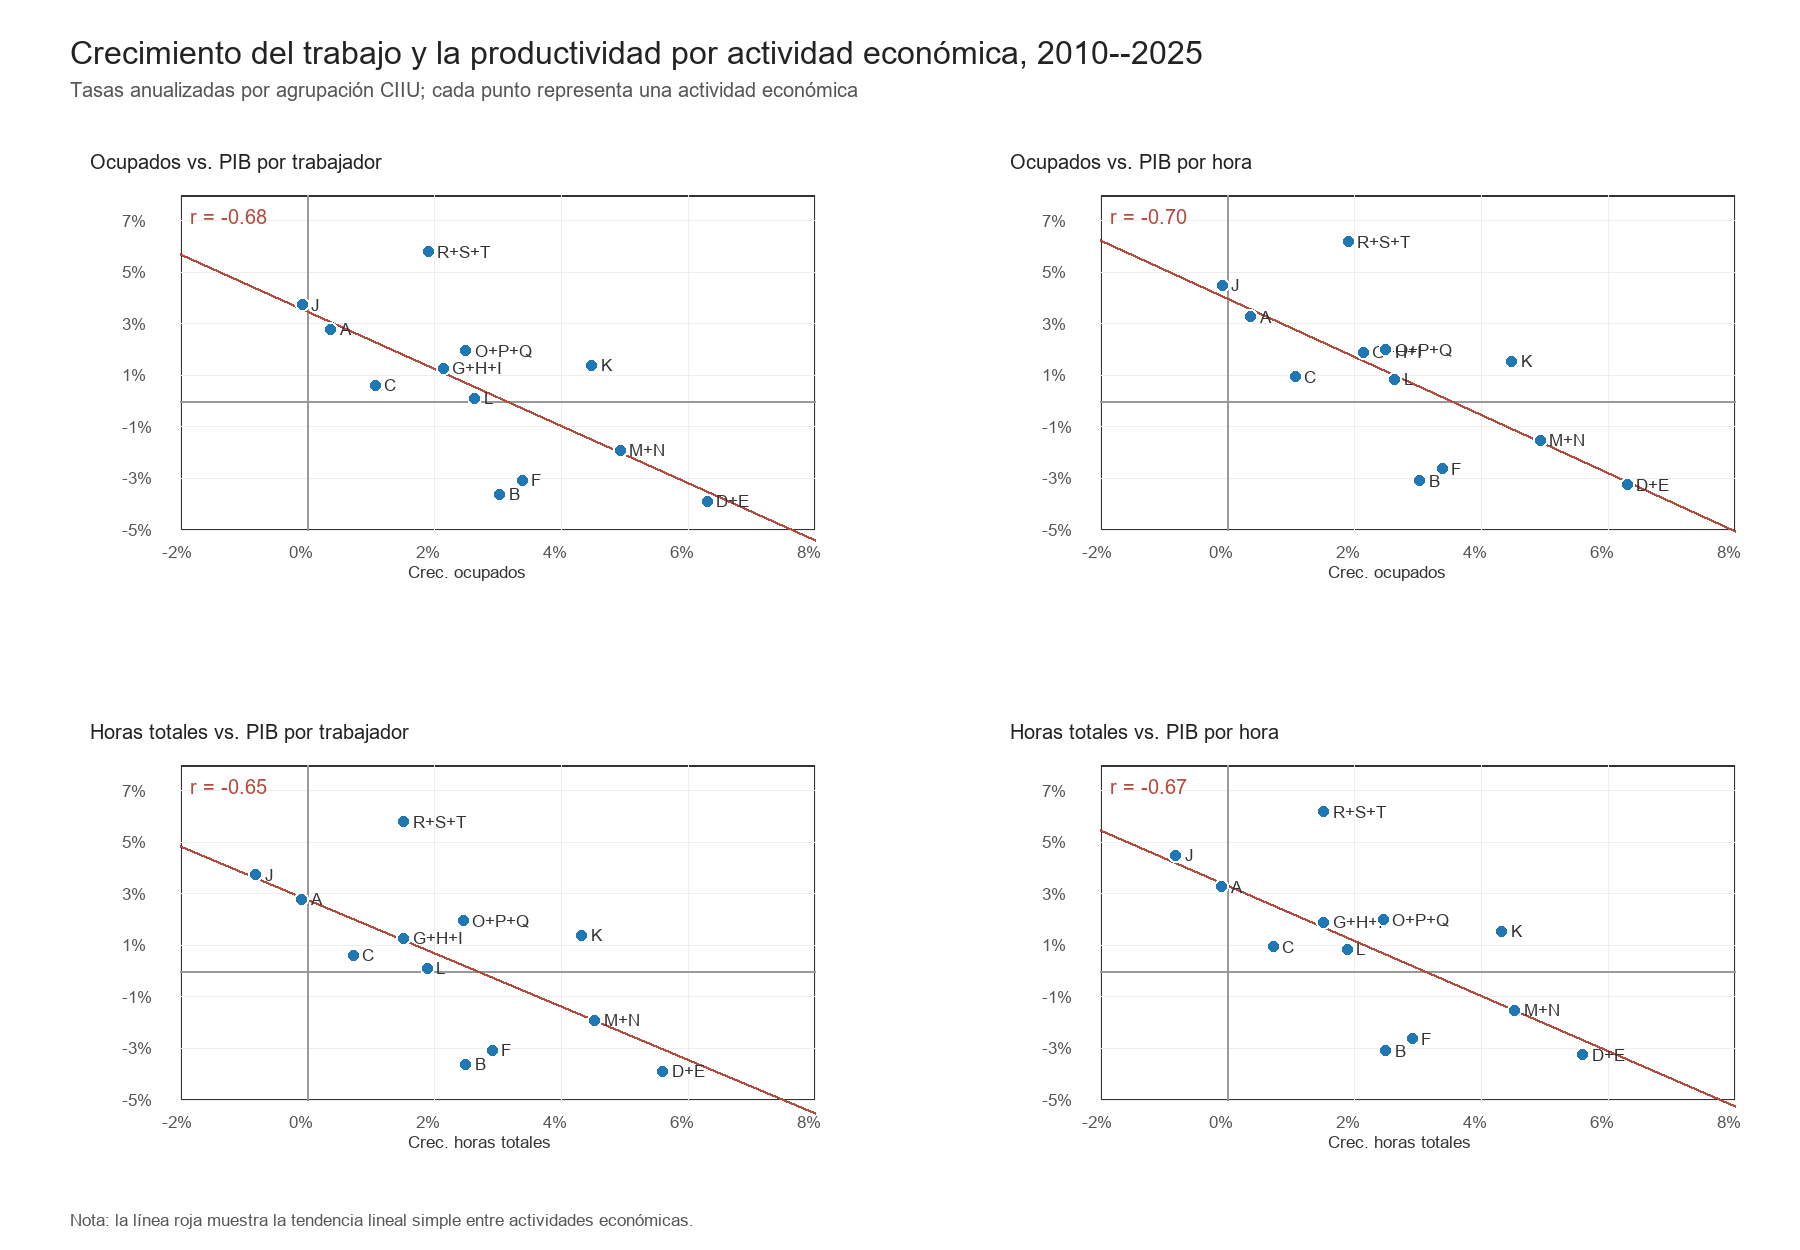
\includegraphics[width=0.95\textwidth]{Paper/figures/fig_pib_geih_productividad_sector_correlaciones.png}
  \caption{Crecimiento sectorial del trabajo y la productividad}
  \label{fig:pib_geih_productividad_sector_correlaciones}
\end{figure}

El patrón transversal entre sectores refuerza la lectura de heterogeneidad. Las ramas donde más crecen los ocupados y las horas totales no son, en promedio, las mismas donde más aumenta la productividad: la correlación entre el crecimiento de los ocupados y el crecimiento del PIB por trabajador es -0,68, y la correlación entre el crecimiento de las horas totales y el crecimiento del PIB por hora es -0,67. Esto no implica que el empleo sea indeseable, sino que la absorción de trabajadores se ha concentrado parcialmente en sectores donde el valor agregado por trabajador crece menos o incluso cae. En contraste, las dos medidas de productividad se mueven casi una a una entre sectores, con una correlación de 0,997, lo que indica que el ranking sectorial de desempeño productivo es muy similar si se mide por trabajador o por hora.

\section{Conclusiones}

El principal resultado del informe es que Colombia aumentó su productividad laboral entre 2010 y 2025, pero lo hizo a un ritmo moderado. El PIB por trabajador creció cerca de 1\% anual, mientras que el PIB por hora trabajada avanzó algo más rápido. Esta diferencia no es un detalle estadístico: refleja que la economía incorporó más ocupados, pero con una reducción de las horas semanales promedio por trabajador. Por eso, medir la productividad por trabajador y por hora permite separar mejor los márgenes detrás del crecimiento económico.

La mirada sectorial muestra que el reto no es solo agregado. Algunos sectores, como información y comunicaciones, agropecuario y artes, otros servicios y hogares, registraron mejoras importantes de productividad. Otros, en cambio, presentaron caídas en el PIB por trabajador y en el PIB por hora. Además, los sectores que más aumentaron sus ocupados no fueron necesariamente los que más elevaron su productividad. Esto no implica que la creación de empleo sea una mala noticia, sino que la calidad productiva de esa absorción laboral importa para que el crecimiento se traduzca en mejores salarios e ingresos.

La agenda de productividad para Colombia debe combinar tres frentes: elevar la productividad dentro de los sectores que concentran empleo, facilitar la reasignación hacia actividades de mayor valor agregado y cerrar brechas de capacidades, tecnología, formalización y gestión empresarial. Este informe ofrece una primera base descriptiva para esa discusión. Los siguientes informes de la serie podrán profundizar en los mecanismos detrás de estas brechas y en las políticas necesarias para convertir crecimiento, empleo y productividad en mejoras sostenidas del bienestar.
